\documentclass{article}
\usepackage[utf8]{inputenc}
\usepackage{float}
\usepackage{graphicx}

\title{Appunti Advanced Networking \\ and Wireless Systems}
\author{}
\date{Marzo - Aprile 2020}

\begin{document}

\maketitle

\tableofcontents

\newpage
\section{IPv6}
Gli indirizzi IPv4 stanno finendo a causa della rapida crescita degli utenti Internet (limite teorico di 4.3 miliardi di indirizzi), quindi perchè IPv6 non è ancora lo standard?
\begin{itemize}
    \item Implica un grande cambiamento nell'infrastruttura di rete.
    \item Infrangerebbe un grande principio del protocollo IP: l'\textit{univocità} degli indirizzi.
    \item Il NAT funziona talmente bene nel risolvere problemi di spazio di indirizzamento IPv4 che fino ad oggi non si è sentito il bisogno di passare a IPv6.
\end{itemize}
Tuttavia le cose ora stanno cambiando: la crescita demografica accoppiata ad una crescente richiesta di accesso ad internet (pensiamo a paesi come Cina ed India) si traducono in una grande richiesta di indirizzi IP nel futuro prossimo.
Inoltre, in futuro, con l'avvento dell'IoT ci saranno numerosi oggetti sempre connessi ad internet (es. sensori domestici) per i quali servirà un indirizzo IP permanente (\textit{always-on-access}).

\subsection{IPv6 Base Header}
\begin{figure}[H]
\centering
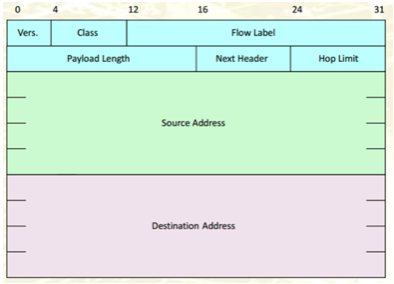
\includegraphics[scale=0.5]{figures/base header.png}
\caption{IPv6 Base Header}
\end{figure}

\begin{itemize}
    \item \textbf{Version} \textit{(4 bits)}: indica che stiamo utilizzando IPv6.
    \item \textbf{Traffic class} \textit{(1 byte)}: sostituisce il campo Type of Service dell’IPv4. Può essere utilizzato per dare priorità a certi a datagram di certe applicazioni (per esempio, pacchetti ICMP) rispetto a datagram di altre applicazioni.
    \item \textbf{Flow label} \textit{(20 bits)}: generato randomicamente. Distingue pacchetti che richiedono stessi trattamenti in modo da facilitare la gestione del traffico real time. E’ considerata una feature sperimentale. Per alcune applicazioni è importante andare a rilevare una sequenza di pacchetti trasmessi da un sender a un receiver. Questo perché i requisiti di un applicazione possono dipendere da alcune metriche di performance che considerano più pacchetti contemporaneamente. Senza la flow label, per identificare pacchetti appartenenti allo stesso flusso si usavano implicitamente gli indirizzi di destinazione e sorgente. Con questo nuovo parametro si può specificare in modo esplicito. Il sender mette lo stesso valore di flow label per i pacchetti che appartengono allo stesso flow, quindi il flusso viene riconosciuto dai router guardando IP Address del sender e flow label Da aggiungere, inoltre, che con il NAT non funzionava, perché il source address cambia (ci possono essere più sender dietro lo stesso NAT con lo stesso indirizzo).
    \item \textbf{Payload length} \textit{(2 bytes)}: non include la lunghezza dell’header, com’era in IPv4. Gli header di estensione sono considerati come parte del payload.
    \item \textbf{Hop limit} \textit{(1 byte)}: Analogo al campo TTL nell’IPv4, ma in questo caso non è espresso in secondi. Quindi, ogni device intermedio prima della destinazione, riduce di uno l’hop limit, se questo arriva a 0 il pacchetto viene scartato.
    \item \textbf{Next header} \textit{(1 byte)}: Assomiglia al tipo di protocollo in IPv4 ma è molto di più, riflette la nuova organizzazione dei pacchetti IPv6.
\end{itemize}

Nell’header dell’IPv4 c’èra IHL (Internet Leader Length) che serviva per comunicare al ricevitore e ai nodi intermedi la lunghezza dell’header, che era variabile per via del campo options di dimensioni variabili. IPv6, invece ha un header di dimensione fissa, il controllo viene fatto via Hardware. 40 Byte. IPv6 non è provvisto di frammentazione. In IPv4, se il pacchetto è più grande di MTU, si frammenta; in IPv6 si droppa. MTU varia a seconda del canale. 1280 è il minimo MTU che si può assumere su un qualunque link di internet. Se si vuole spedire di più, bisogna stimare MTU lungo il path. 

\section{IPv6 Header Structure}
Un Base Header (40 bytes), più zero o più extension headers di dimensione variabile.

\begin{figure}[H]
\centering
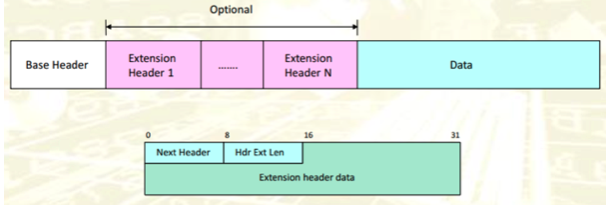
\includegraphics[scale=0.5]{figures/header structure.png}
\caption{IPv6 Header Structure}
\end{figure}

Ogni extension contiene una sola feature e tutti i dati necessari a questa feature.Next header contiene le informazioni sul tipo di dati contenuti nel successivo header. Header extensions length contiene la lunghezza dell’header, in pratica contiene un puntatore alla prossima estensione. \\ Quindi, ogni extension header può essere considerato come un sotto-protocollo che svolge una nuova funzione. E’ possibile che in un extension header sia contenuto un altro pacchetto IPv6: questa tecnica è chiamata “tunneling”. \\ Valori nel campo “Next Header” (base e extension):

\begin{figure}[H]
\centering
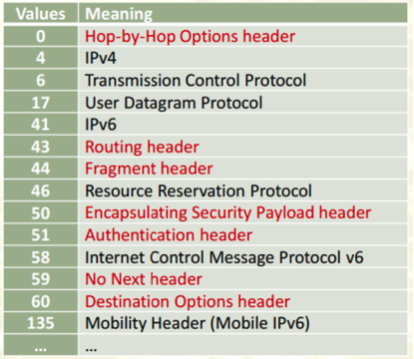
\includegraphics[scale=0.5]{figures/next header values.png}
\caption{IPv6 Next Header Values}
\end{figure}

Gli extension headers vengono inseriti solo quando è necessario. Sono processati nell’ordine in cui appaiono dal nodo identificato dal destination address. \\ Valori che può assumere il campo Next Header:

\begin{figure}[H]
\centering
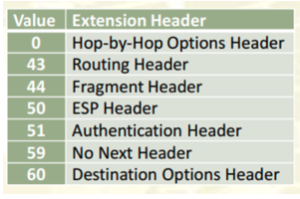
\includegraphics[scale=0.5]{figures/next header used.png}
\caption{IPv6 Next Header Values used}
\end{figure}

I valori “ESP header” e “Authentication Header” servono per sicurezza, autenticazione ed encryption. Valore “No next Header” serve a specificare che non c’è nient’altro nel pacchetto dopo. \\ La regola generale è che il base header venga processato da ogni dispositivo intermedio da cui passa il pacchetto (ogni router del percorso più la destinazione). Mentre gli extension header vengono lette solo a destinazione. L’unica eccezione riguarda l’ “hop by hop options header”.\\ Il “processare un header” si riferisce al fatto che il payload viene mandato al livello superiore. \\ Solitamente si rispetta un ordine, ovvero il “routing header” deve essere prima del “fragment header”.

\subsection{Hop-by-Hop Options header}
Porta informazioni opzionali che devono essere esaminate da ogni nodo sul cammino (hop-by-hop).\\ Se il pacchetto contiene più extension headers, questo deve essere il primo.\\ Formato:

\begin{figure}[H]
\centering
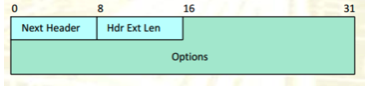
\includegraphics[scale=0.5]{figures/hopbyhop format.png}
\caption{Hop-by-Hop Option Header Format}
\end{figure}

\begin{itemize}
    \item \textbf{Next Header} \textit{(1 byte)}
    \item \textbf{Header Extension Length} \textit{(1 byte)}
    \begin{itemize}
        \item Lunghezza dell’header in unità di otto byte (meno 1)
    \end{itemize}
    \item \textbf{Options}: una o più
\end{itemize}

Per quanto riguarda il campo Options:
\begin{figure}[H]
\centering
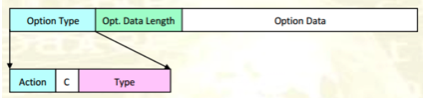
\includegraphics[scale=0.5]{figures/option field.png}
\caption{Option field}
\end{figure}

\begin{itemize}
    \item \textbf{Action} \textit{(2 bits)}: Cosa fare se l'opzione non è riconosciuta
    \begin{itemize}
        \item \textbf{00}: Salta e continua a processare.
        \item \textbf{01}: Scarta il pacchetto.
        \item \textbf{10}: Scarta il pacchetto e manda un messaggio ICMP Parameter Problem all’indirizzo Source del pacchetto.
        \item \textbf{11}: Scarta il pacchetto e manda un messaggio ICMP Parameter Problem all’indirizzo Source del pacchetto solo se la destinazione non è un indirizzo multicast
    \end{itemize}{}
    \item \textbf{C} \textit{(1 bit)}
    \begin{itemize}
        \item \textbf{1}: l’informazione di opzione può cambiare in viaggio
        \item \textbf{0}: l’informazione di opzione non cambia in viaggio
    \end{itemize}
    \item \textbf{Type}
    \begin{itemize}
        \item \textbf{Jumbo Payload} \textit{(Type = 194)}:   Utilizzato per inviare pacchetti molto grandi la cui lunghezza non può essere codificata su soltanto 16 bits (>64 KB). \\ Quando viene utilizzato, il campo length del payload IPv6 è settato a 0. \\ La lunghezza del pacchetto è codificata con 32-bits, supporta la trasmissione di pacchetti che stanno tra 65.536 e 4.294.967.295 bytes (4GB).\\ Compromesso tra il design iniziale di IPv6 e requirements speciali di networking. \\ Quindi, le informazioni del payload non vengono messe all’interno della sezione payload ma all’interno dell’estensione.
        \item \textbf{Router Alert} \textit{(Type = 5)}: Indica ad un router sul cammino di forwarding che il pacchetto contiene informazioni importanti che devono essere processate dal router.\\ Esempio: RSVP utilizza pacchetti di controllo che contengono informazioni che hanno bisogno di essere interpretate o aggiornate da routers sul cammino.
    \end{itemize}
\end{itemize} 

\subsection{Routing Header}
Definisce una lista di nodi intermedi che devono essere visitati sul cammino alla destinazione
\begin{itemize}
    \item \textbf{Routing Type}
    \begin{itemize}
        \item 0: default
        \item 2: Mobile IPv6
        \item 3: RPL
    \end{itemize}
    \item \textbf{Segment Left}: nodi rimanenti che devono essere visitati
    \item \textbf{Address} (RT = 0)
\end{itemize}
Di solito non si ha il controllo sulla route utilizzata per raggiungere la destinazione finale. Per avere il controllo sul path si usa questa estensione, dove si indica la lista dei router che si vuole che vengano attraversati per consegnare il pacchetto. Non si vanno a rimuovere via via i routers, cosicché il destinatario può sapere il percorso fatto dal pacchetto per raggiungerlo. Non si tiene però conto, in questo modo, del fatto che uno di questi router potrebbe essere congestionato. Soluzione: loose control, ovvero non si specifica tutta la lista ma solo un hop dal quale attraversare. \\ A volte è necessario costruire router senza routing table. Rilevante nelle capillary network dove il router potrebbe essere un sensore. Accade ad esempio in RPL (Routing protocol for low power and lossy network). Un problema è legato al fatto che alcuni nodi intermedi potrebbero essere malevoli e leggere i pacchetti che poi verranno inoltrati. Un altro possibile problema riguarda il DoS attack: ovvero si possono modificare gli indirizzi dei nodi intermedi e far convergere tutto il traffico verso un solo nodo. Per questo motivo adesso questo header è deprecato.

\subsection{Fragment Header}
Diversamente da IPv4, i routers non frammentano pacchetti IPv6.
La frammentazione avviene solo all’host sorgente, che manda il pacchetto. L’host di destinazione gestisce semplicemente il riassamblamento. I pacchetti IPv6 più larghi dell’MTU sul link di forwarding sono scartati dal router. \\
Gli host IPv6 utilizzano una procedura di discovery di cammini MTU.
La minima grandezza IPv6 MTU è 1280 bytes. \\ Questo header viene usato dal sender nel caso voglia frammentare il pacchetto. Solo il sender può usare la frammentazione e il ricevente si preoccupa di ricollegare i pacchetti frammentati. I nodi intermedi non usano frammentazione, inoltrano solo gli stessi pacchetti. \\ Per definizione un link in cui si usa IPv6 deve garantire un minimum MTU pari a 1280 bytes, per cui se un sender manda un pacchetto di dimensione minore a 1280 bytes saprà con certezza che il pacchetto arriverà a destinazione senza essere scartato o frammentato dai router lungo il path. E se un sender volesse mandare pacchetti più grandi di 1280 bytes, deve usare la path MTU discovery per scoprire se lungo il cammino è disponibile un MTU maggiore di 1280 bytes, oppure lo stesso sender può usare la frammentazione. \\ Path MTU discovery procedure: in questa procedura si usa ICMPv6 per scambiarsi informazioni riguardo l’MTU. Per scoprire la minima MTU si manda un pacchetto di una certa dimensione e se non riceviamo in risposta nessun errore ICMPv6, allora l’MTU minimo è sicuramente maggiore della dimensione del pacchetto. Se il minimo MTU è minore, il router scarterà il pacchetto e manderà un pacchetto ICMPv6 di errore al sender con all’interno il valore del minimo MTU.
Se un link non è in grado di garantire una MTU di 1280 bytes, allora non potrà utilizzare IPv6 (sarà un problema con IoT).

\begin{figure}[H]
\centering
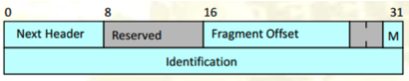
\includegraphics[scale=0.5]{figures/fragment header.png}
\caption{Fragment Header}
\end{figure}

\begin{itemize}
    \item \textbf{Fragment Offset} \textit{(13 bits)}: L’offset in unità di 8 byte del dato in questo pacchetto relativo all’inizio del dato nel pacchetto originale.
    \item \textbf{M-Flag} \textit{(1 bit)}:
    \begin{itemize}
        \item 1: più frammenti
        \item 0: ultimo frammento
    \end{itemize}
    \item \textbf{Identification} \textit{(4 bytes)}: Generato dall’host sorgente in modo da identificare tutti i pacchetti che appartengono al pacchetto originale.
\end{itemize}

\subsection{Altri Extension Headers}
\begin{itemize}
    \item Authentication Header
    \item Encapsulating Payload Security Header \\
    IPv6 security support (IPsec)
    \item No Next Header: No Payload
    \item Destination Options Header \\
    Lo stesso di Hop-by-Hop, ma le opzioni devono essere processate solo alla destinazione. \\
    Utilizzato dal Mobile IPv6
\end{itemize}

\section{Categorie di indirizzi}
\begin{itemize}
    \item \textbf{Unicast}: identifica in maniera univoca un’interfaccia di un nodo IPv6. Un pacchetto inviato ad un indirizzo unicast è inviato all’interfaccia identificata da quell’indirizzo.
    \item \textbf{Multicast}: identifica un gruppo di interfacce IPv6. Un pacchetto inviato ad un indirizzo multicast è processato da tutti i membri del gruppo multicast.
    \item \textbf{Anycast}: assegnato a interfacce multiple (tipicamente su nodi multipli). Un pacchetto inviato ad un indirizzo anycast è consegnato a soltanto una di queste interfacce (tipicamente la più vicina).
\end{itemize}

Non è presente il broadcast in IPv6. Il broadcast veniva usato in IPv4 con DHCP ad esempio. Il Broadcasting in IPv4 è limitato alla stessa subnet (rete locale, ovvero il router non manda verso l’esterno i pacchetti broadcast). \\
In IPv6 si utilizzano di default dei Multicast address per identificare il servizio necessario. Questo indirizzo sarà associato al server che svolge quel servizio, quindi tutti i server DHCP avranno lo stesso indirizzo multicast IPv6. In questo modo il pacchetto viene ricevuto solo dal server DHCP e tutti gli altri nodi non interessati (dato che non forniscono quel servizio) non riceveranno il messaggio, non dovranno quindi processarlo per poi scartarlo (come in IPv4).\\
Un indirizzo IPv6 è assegnato ad un’interfaccia, almeno un indirizzo unicast per interfaccia di un nodo. Una singola interfaccia può essere assegnata a più indirizzi IPv6 di ogni tipo. 
Gli indirizzi IPv6 hanno uno “scope” (codificato come parte dell’indirizzo): lo “scope” è un intervallo topologico tra cui gli indirizzi potrebbero essere usati come identificatori unici. E’ una parte dell’indirizzo che indica la parte della rete dove l’indirizzo può essere usato come unico.
Ci sono scope globali e non globali.\\
Non è più presente ARP, il servizio viene fornito direttamente da IPv6. Scope è un sottoinsieme di tutta la network codificata con un indirizzo.
In IPv4 c’è solo uno scopo, che è il global-scope, mentre in IPv6 c’è sia il global-scope che local-scope.

\subsection{Link IPv6}
Identificato da un set di interfacce che possono comunicare direttamente tra di loro (hop singolo). Un link IPv6 è un’astrazione, insieme di interfacce che possono comunicare direttamente senza l’intermezzo di un router. 
Il protocollo IP introduce un modello per modellare la rete. Un link che pensiamo come ad esempio un filo, è in realtà un'astrazione di ciò che il sottostante link-layer protocol permette di fare. Se, per esempio, si dice che un link è broadcast, significa che la sottostante link-layer technology mette a disposizione di IP la comunicazione broadcast (non si parla quindi del mezzo). \\
Ethernet supporta broadcast, la tecnologia però, non lo è. È connessa a degli switch in unicast (point-to-point).
Tipiche assunzioni riguardo ad un link:
\begin{itemize}
    \item Stabile (nel tempo)
    \item Single link-layer broadcast domain
    \item Transitive (se A-B e B-C, allora A-C)
\end{itemize}{}
Implicazioni:
\begin{itemize}
    \item I prefissi network possono essere usati per determinare se un'interfaccia è attaccata ad un certo link.
    \item La rilevazione di indirizzi duplicati può essere facilmente indirizzata
\end{itemize}{}
Se non vale la proprietà transitiva, non si può usare la on-link determination. Quindi, il discorso è che le funzionalità che otteniamo ad un determinato livello (in questo caso 3, IPv6) dipendono da cosa ottieni dai livelli sottostanti.\\
La transitività riguarda i link unicast, non broadcast. Se un link è broadcast puoi far girare una procedura (duplicate address detection - stateless address autoconfiguration) per controllare se ci sono altri nodi sullo stesso link che utilizzano lo stesso indirizzo che si vuole assegnare.

\subsection{Address Scope}
\begin{itemize}
    \item \textbf{Global Address scope}: unico nell'intera internet
    \item \textbf{Link-local}: Assomiglia vagamente ai private address di IPv4, ma è più specifico. Grazie al link-local address ed al fatto che gli host possono autoconfigurare le proprie interfacce, la comunicazione su un link può avvenire senza bisogno di altro, senza bisogno di un gestore.\\
    L'indirizzo quindi è unico sul link al quale è attaccata l'interfaccia corrispondente. 
    \item \textbf{Unique local}: Indirizzo globally unique, ma valido solo in un sottoinsieme dei link. Non dovrebbe essere "routato" nel global Internet.\\ In IPv4 c'erano gli indirizzi privati, come 192.168.0.1: questa soluzione non garantisce unicità globale: collegando 2 reti si hanno conflitti di indirizzi.
\end{itemize}{}

\subsection{Notazione di indirizzi}
\textbf{x:x:x:x:x:x:x:x} dove x è un blocco da 16bit rappresentato da 4 cifre esadecimali.\\ Regole di abbreviazione:
\begin{itemize}
    \item Zeri iniziali possono essere saltati
    \item Zeri consecutivi possono essere sostituiti da "::" e questa regola può essere applicata soltanto una volta, altrimenti non sapresti la dimensione dei blocchi rimossi
\end{itemize}{}
L'indirizzo con tutti 0: \textbf{0:0:0:0:0:0:0:0} (::) indica un indirizzo non specificato.\\ L'indirizzo \textbf{0:0:0:0:0:0:0:1} (::1) indica l'indirizzo loopback, ovvero corrisponde al localhost in IPv4.

\subsection{Prefissi: notazione e allocazione}
Simile all'IPv4 con CIDR: [Indirizzo IPv6]/[lunghezza prefisso].\\
Identifica un set di indirizzi che, ad esempio, possono appartenere alla stessa subnet.

\begin{figure}[H]
\centering
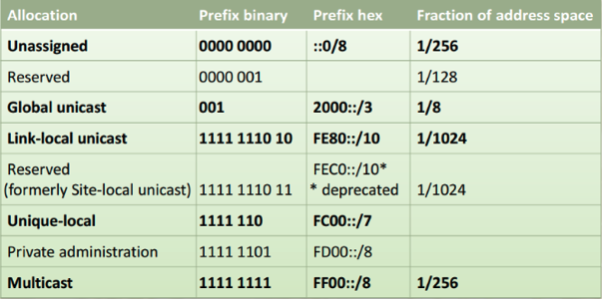
\includegraphics[scale=0.5]{figures/prefix notation.png}
\caption{Allocazione dei prefissi}
\end{figure}

\subsubsection{Global Unicast}

\begin{figure}[H]
\centering
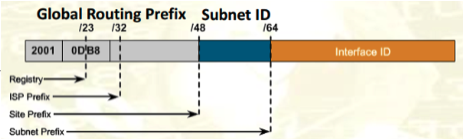
\includegraphics[scale=0.5]{figures/global unicast.png}
\caption{Global unicast address}
\end{figure}

Il prefisso Global Routing identifica il range di indirizzi allocati ad un luogo. Questa divisione è un possibile uso; l'unica cosa obbligatoria è avere una parte per la rete (subnet) e una parte per l'interfaccia. Questo boundary è 64, la divisione è fissata.

\paragraph{Interface ID}
Perché si hanno così tanti bit per l'Interface ID? In IPv4, ad esempio, si hanno $2^{8}-1$ indirizzi assegnabili manualmente o automaticamente, ad esempio tramite un server DHCP. \\ L'idea in IPv6, è fare un'implementazione di questa operazione completamente stateless. Cosa si intende per stateless? E' un pezzo di informazione memorizzato da qualche parte, che sia sul nodo (configurazione manuale) o sul DHCP server. La fai usando il link-layer address. Non c'è uno "state" al livello 3. Il link-layer address è univoco, perché IEEE gestisce lo spazio di indirizzi. È diviso in 2 parti. L'univocità della prima parte in base al produttore, è garantito da IANA, mentre la parte rimanente dipende dal produttore. Si suppone che sia univoco, a livello link-layer. \\ Questa specifica è stata estesa a 64 bit, per questo in IPv6 si usano 64 bit per l'interface ID: tali bit corrisponderanno al link-layer address. \\ Ci sono regole per passare da 48 a 64 bit:

\begin{figure}[H]
\centering
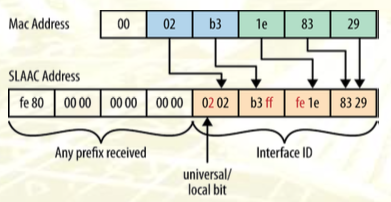
\includegraphics[scale=0.5]{figures/64-48 conversion.png}
\caption{Conversione da 48 a 64}
\end{figure}

\textit{SLAAC = Stateless Address AutoConfiguration} \\ Si aggiungono le parti rosse indicate in figura. Adesso, ogni interfaccia può comunicare il proprio Interface ID. \\ Si crea un problema: si può identificare il dispositivo indipendentemente da dove ti colleghi: per questo, infatti, ci sono diversi modi per generare l'ID dell'interfaccia. 

\subparagraph{Problema della privacy}  
L'accesso ad Internet potrebbe essere tracciato anche tra networks, questo perché l'identificatore è univoco tra le interfacce. 
\begin{itemize}
    \item \textbf{Stable privacy addresses:} Non è basato su un identificatore hardware, viene generato in modo random. Non cambia all'interno di una subnet, ma cambia quando l'host si muove da un network all'altro.
    \item \textbf{Temporary transient:} Assegnato utilizzando un numero random che cambia ad intervalli regolari.
\end{itemize}

\paragraph{Indirizzi link-local e local}
Gli indirizzi link-local sono assegnati di default attraverso auto-configurazione. L'ID Globale di indirizzi univoci IPv6 è generato randomicamente.

\begin{figure}[H]
\centering
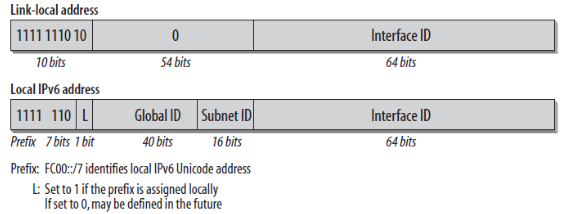
\includegraphics[scale=0.5]{figures/linklocal.png}
\caption{Indirizzi link local}
\end{figure}

I 64 bit finali sono quelli generati nei modi spiegati precedentemente (Interface ID). \\ Prefisso: FC00::/7 identifica gli indirizzi locali IPv7 Unicode. \\ Il bit L è settato a 1 se il prefisso è assegnato localmente e se settato a 0, potrebbe essere definito in futuro.

\subsubsection{Indirizzi Anycast}
Un indirizzo Anycast è assegnato ad interfacce multiple (tipicamente su nodi multipli). Un pacchetto inviato ad un indirizzo anycast è consegnato a soltanto una di queste interfacce (tipicamente la più vicina). \\ Progettato per fornire ridondanza e bilanciamento del carico quando lo stesso servizio è fornito da host o router multipli, come nel caso del DNS. \\ Sappiamo che i nomi in internet hanno una gerarchia ed abbiamo una corrispondente gerarchia di server. Il root server è sempre lo stesso, è un server solo. Servirebbe l'indirizzo dei server, una lista di server; in questo caso si può utilizzare un indirizzo anycast, virtualmente assegnato a tutte le copie del server. Delego alla rete il compito di scegliere il root DNS server giusto. Quindi, il DNS è una routing functionality. \\ Si deve far attraversare ad un pacchetto un autonomous system, se c'è un indirizzo anycast associato con quell'autonomous system, allora sicuramente il pacchetto eventualmente sarà consegnato ad uno dei border router dell'AS. E' implementato come una funzionalità di routing. Per ottenere questo comportamento basta che nella routing table ci sia un'entrata per quello specifico indirizzo. Se è IPv4, significa che si avrà una entry /32 nella tabella di routing: se l'indirizzo di destinazione matcha esattamente questo indirizzo, allora il prossimo hop è questo. Se c'è un'entrata IPv6 /128, questa entrata sarà usata solo come la prima: è il prefisso più lungo che puoi avere. Con questo meccanismo si può quindi andare a stabilire il path che verrà seguito dai pacchetti che fanno match con tale indirizzo. Non c'è bisogno, quindi, di identificare un indirizzo come anycast: un indirizzo anycast è più una funzionalità di routing che un tipo di indirizzo (è l'IP routing che decide dove spedire il pacchetto). Un indirizzo anycast non può essere usato con TCP, dal momento che non c'è controllo sulla consegna, funziona bene con UDP. Il sender quindi, non ha controllo sull'interfaccia al quale il pacchetto sarà spedito. \\ L'indirizzo anycast subnet-router è un indirizzo anycast richiesto:

\begin{figure}[H]
\centering
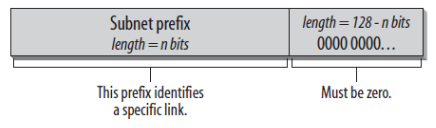
\includegraphics[scale=0.5]{figures/subnet anycast.png}
\caption{Subnet Anycast Address}
\end{figure}

E' associato a tutti i router su una specifica sottorete. Non conosco l'interface ID, altrimenti non sarebbe anycast. Si utilizza ad esempio in Mobile IP.

\subsubsection{Indirizzi Multicast}
Quando un pacchetto è inviato a un indirizzo multicast, tutti i membri del gruppo multicast processano il pacchetto. Un nodo può appartenere a più di un gruppo multicast.

\begin{figure}[H]
\centering
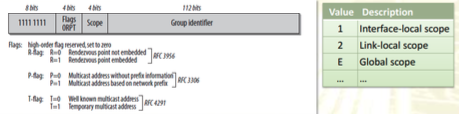
\includegraphics[scale=0.5]{figures/multicast address.png}
\caption{Multicast Address}
\end{figure}

I primi 8 bit sono tutti a 1, poi ci sono 4 bit di flag e 4 bit che indicano lo scope. Non si ha un Interface ID, ma abbiamo un identificativo per un gruppo di interfacce.

\begin{figure}[H]
\centering
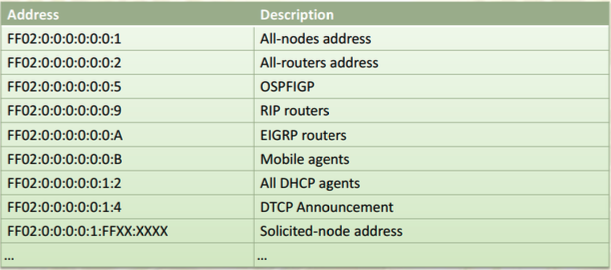
\includegraphics[scale=0.4]{figures/indirizzi tipici multicast.png}
\caption{Indirizzi tipici Multicast}
\end{figure}

\section{ICMPv6 e Autoconfigurazione}
In questa sezione ci sono i veri cambiamenti rispetto ad IPv4: molti protocolli che prima erano "satelliti" ora sono parte di IPv6. Un esempio è ARP: non è una traduzione, ma un'operazione di discovery, di lookup. 

\subsection{ICMPv6} 
\paragraph{Internet Control Message Protocol v6}
Basato sulla versione ICMP di IPv4, con le dovute modifiche per adattarsi al nuovo protocollo. Fornisce funzioni diagnostiche e di gestione dell'errore.\\
I messaggi ICMPv6 sono incapsulati in pacchetti IPv6 con il valore \textit{Next Header 58}. Questa nuova versione fornisce anche una nuova funzionalità denominata \textit{Neighbour Discovery Protocol}, che offre procedure per:
\begin{itemize}
    \item Trovare i router.
    \item Risoluzione di indirizzi a livello collegamento (\textit{livello 2}).
    \item Rilevare possibili indirizzi duplicati.
\end{itemize}
Nella versione IPv4 si poteva tener traccia della raggiungibilità dei vicini solo grazie ad ARP.\\ Il protocollo consiste in un set di operazioni:
\begin{itemize}
    \item Router Discovery
    \item Address Resolution
    \item Duplicate Address Detection
\end{itemize}

\subsubsection{Formato del messaggio}
Come già accennato, questo protocollo genera messaggi che sono trasmessi come payload IPv6 con extension number 58, che identifica ICMPv6.
\begin{figure}[H]
\centering
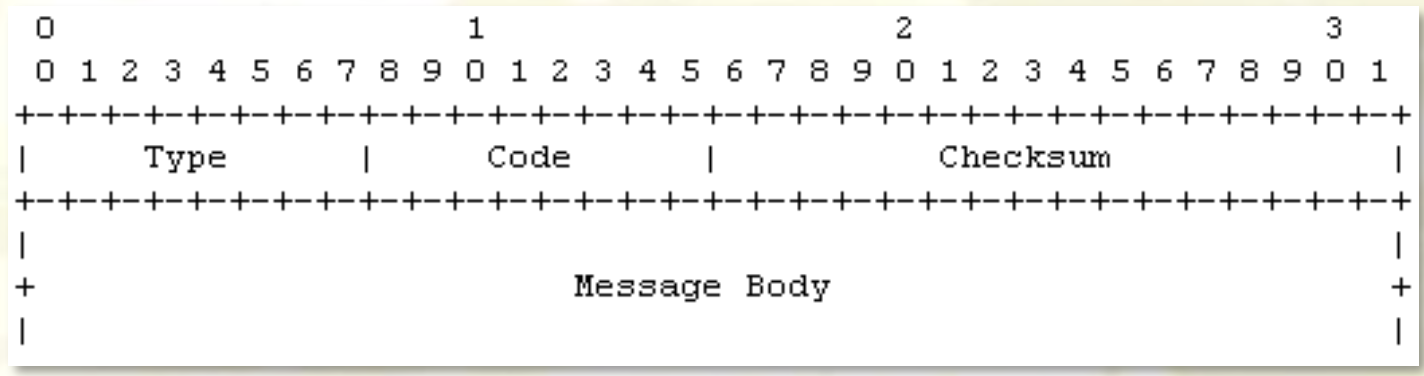
\includegraphics[scale=0.4]{figures/ICMP format.png}
\caption{Formato messaggio ICMP}
\end{figure}
Nel messaggio si possono riconoscere i seguenti campi:
\begin{itemize}
    \item \textbf{Type \& Code}:
        \begin{itemize}
            \item Type = 1, Code = 0: Destinazione non raggiungibile. Quindi, quando un router non ha una route per una certa destinazione, manda indietro al trasmettitore questo ICMPv6.
            \item Type = 2: Pacchetto troppo grande. Questo può servire in un protocollo per scoprire il minimo MTU in un path; viene quindi usato nella fase di path MTU discovery e nel body del messaggio viene inserito l'effettivo MTU.
            \item Type = 3: Time exceeded. Viene usato quando scade l'hop counter del pacchetto
            \item Type = 4: Parameter problem. Usato quando un router rileva problemi nel formato del pacchetto.
        \end{itemize}{}
    \item \textbf{Checksum}: Utilizzato per controllare se il messaggio è corrotto. Questi 2 byte sono necessari, dato che IPv6 non ha nessun meccanismo di checksum. ICMPv6 lavora ad un livello più alto di IPv6, quindi ha bisogno del checksum per controllare che il messaggio non sia corrotto.
    \item \textbf{Corpo del messaggio}: Qua ci va l'informazione vera e propria che trasporta il messaggio. 
\end{itemize}
\begin{figure}[H]
\centering
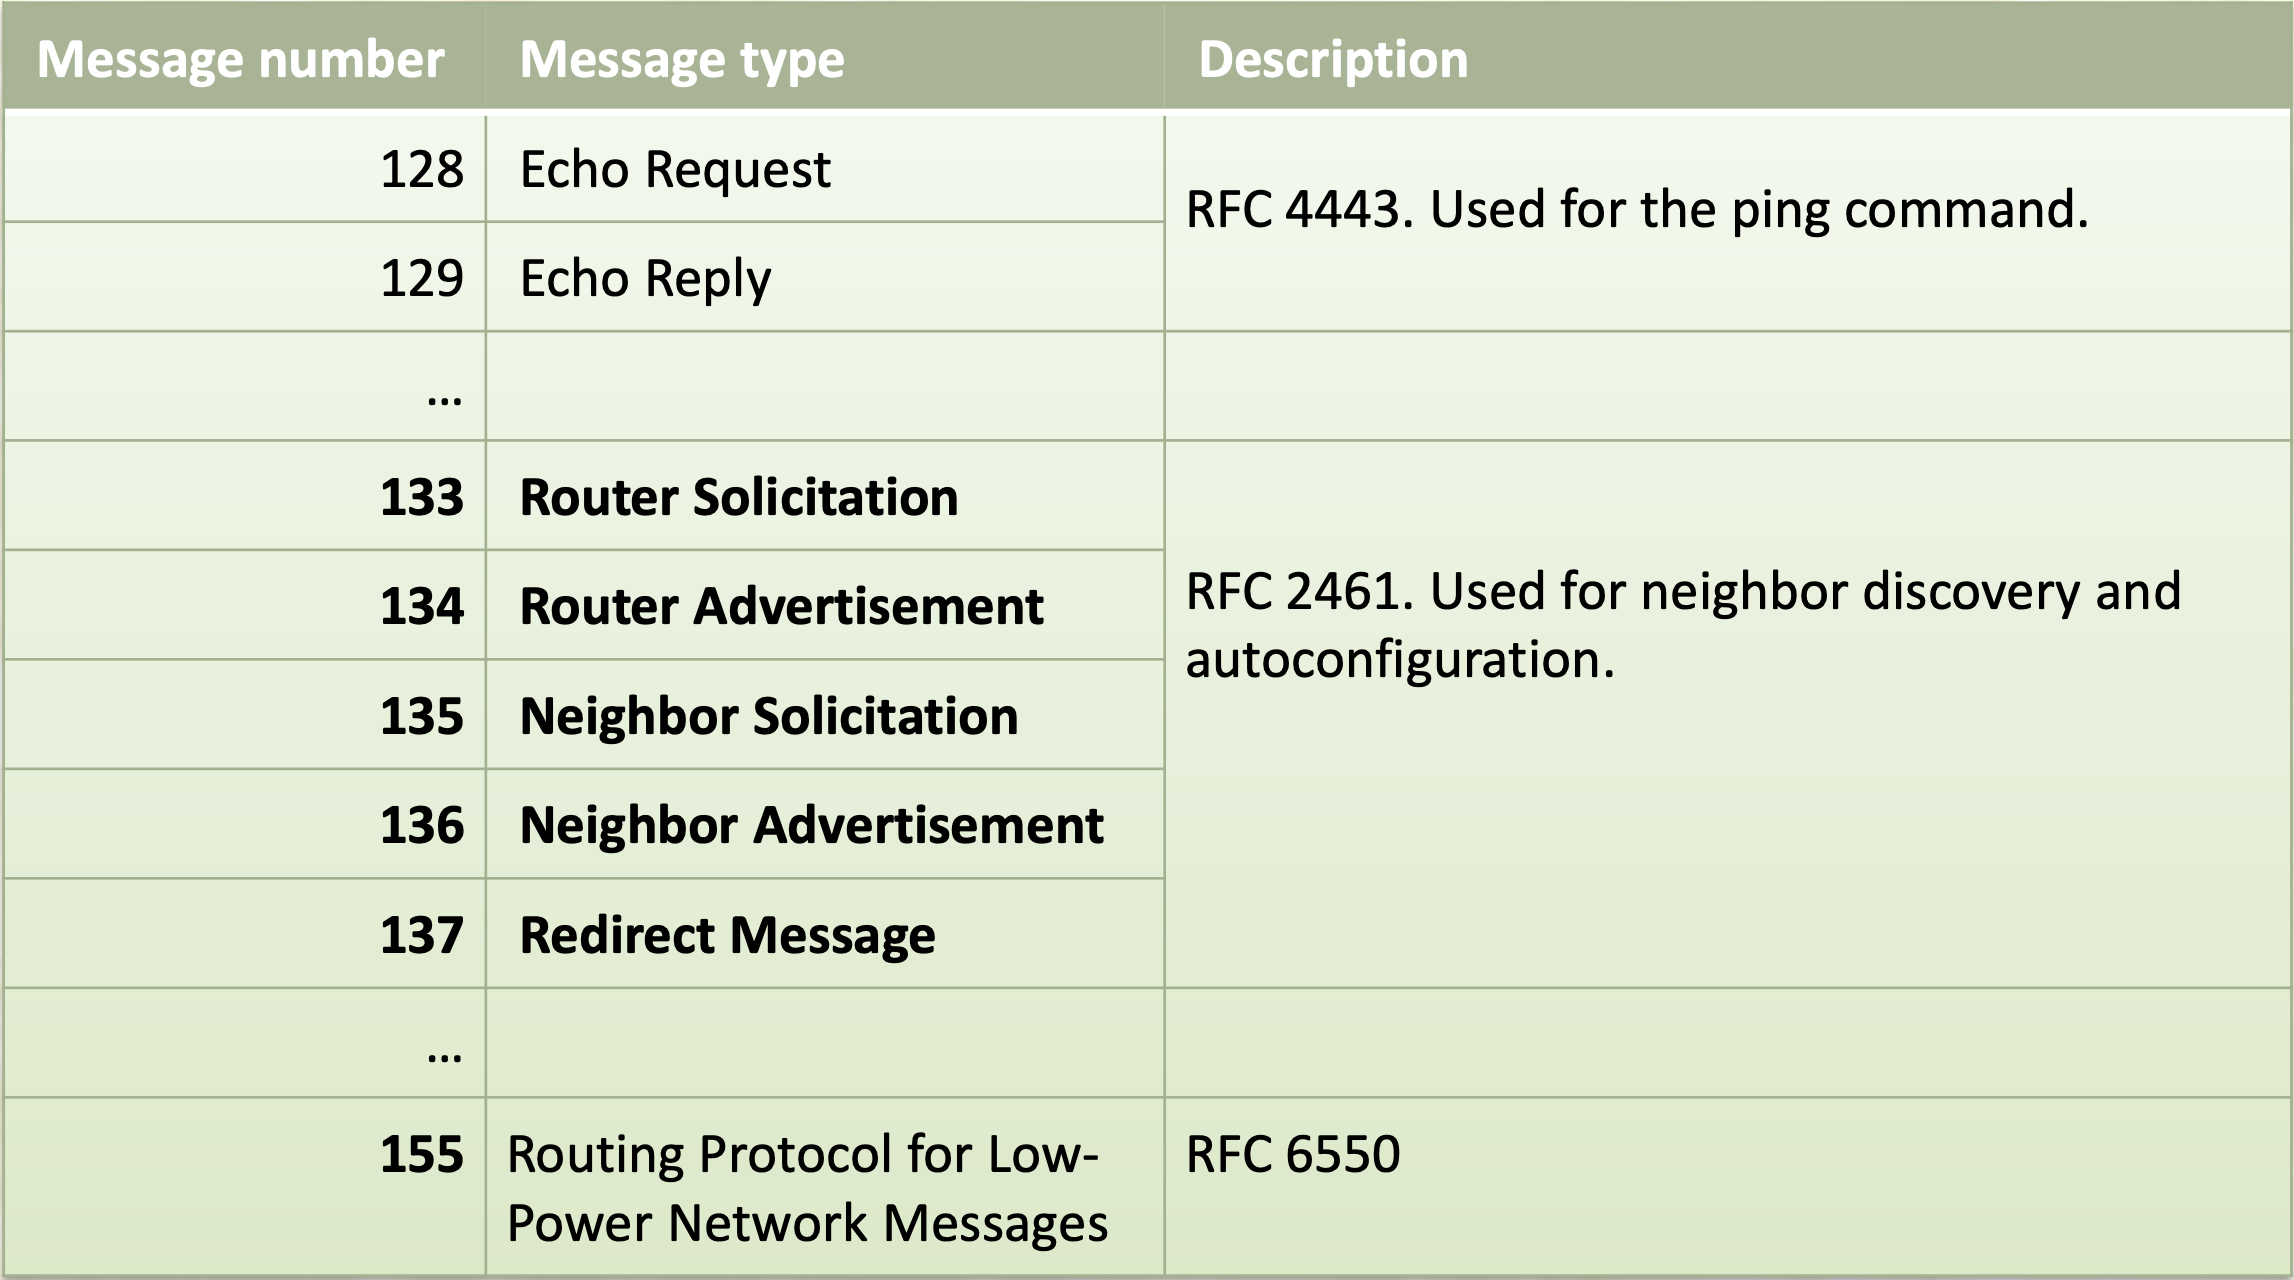
\includegraphics[scale=0.3]{figures/tipi ICMP.png}
\caption{Tipi di messaggio ICMP}
\end{figure}

\subsubsection{Neighbour Discovery protocol}
E' una procedura definita interamente all'interno di ICMPv6 in modo da soddisfare varie feature:
\begin{itemize}
    \item Address Resolution: è un set di funzioni che servono a risolvere un indirizzo IP in un indirizzo layer 2. Sostanzialmente possono verificarsi 2 casi:
    \item Stateless Address Autoconfiguration (SLAAC)
    \item Router Discovery (RD)
    \item Neighbour Unreachability Detection (NUD): per scoprire se qualche vicino non è più raggiungibile
    \item Duplicate Address Detection (DAD)
    \item Redirection
\end{itemize}
Alcune di queste funzionalità sono disponibili anche per IPv4, ma sono implementate in protocolli differenti da IP e ICMP: ad esempio address resolution implementata con ARP. Altre funzionalità, invece, sono nuove come ad esempio SLAAC ed RD.


\subsubsection{Router Discovery}
Periodicamente, i router inviano dei messaggi di \textit{Router Advertisement} all'indi-\\rizzo \textit{multicast all nodes} (codice FF02::1). Questi messaggi contengono le informazioni necessarie ad un host che si vuole unire alla rete per autoconfigurarsi sulla stessa. I RA possono essere richiesti esplicitamente da un nodo tramite un messaggio \textit{Router Solicitation}, sempre all'indirizzo multicast (codice FF02::2).
\begin{figure}[H]
\centering
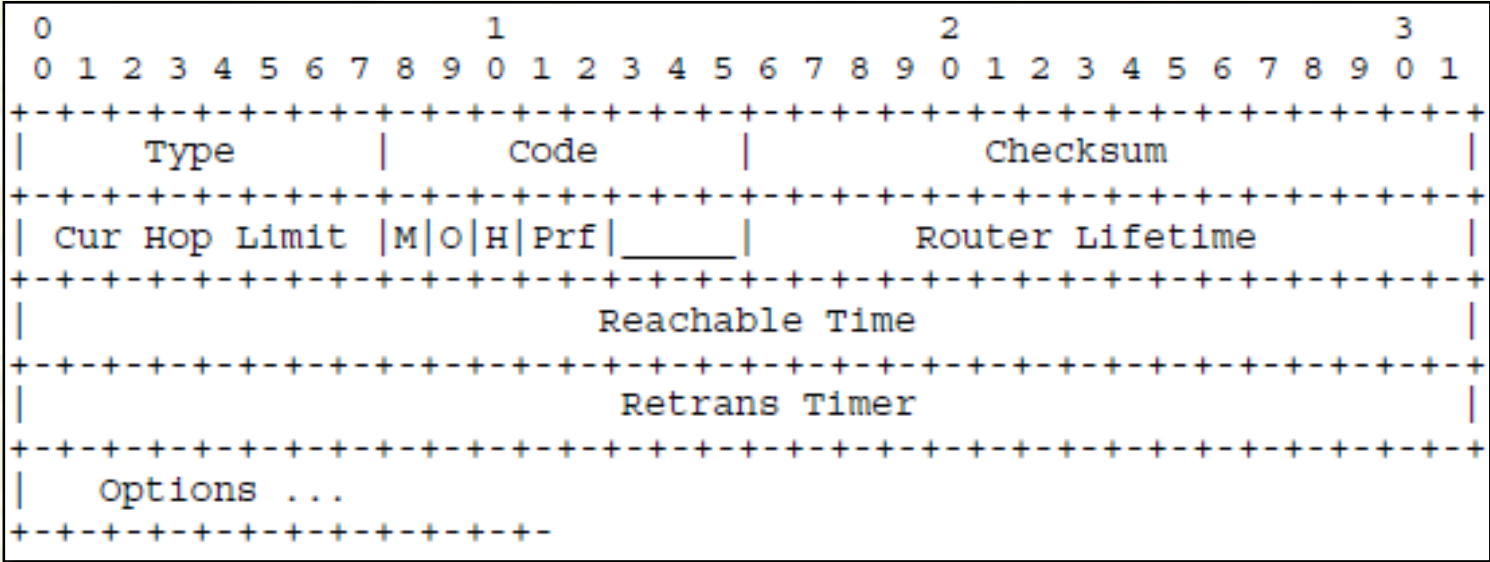
\includegraphics[scale=0.3]{figures/router discovery.png}
\caption{Messaggio router discovery}
\end{figure}
Si vanno ora ad analizzare alcuni campi all'interno del messaggio di Router Advertisement:
\begin{itemize}
    \item Type = 134, Code = 0
    \item Cur Ho Limit: c'è un valore di default per hop limit. Non si può, però, usare un hop limit minore del diametro della nostra rete altrimenti, ovviamente, i pacchetti non arriverebbero al confine. Mentre, non ci sono motivi per impostare un hop limit maggiore del diametro della nostra rete.
    \item Time: parametro di configurazione.
    \item M flag (1 bit): 
        \begin{itemize}
            \item 0: configurazione stateless: in cui si indica che ci deve essere una configurazione autonoma.
            \item 1: configutazione stateful (DHCP): in questo caso non si può scegliere da soli il proprio indirizzo. Si utilizza il servizio DHCP.
        \end{itemize}
    \item Prf flag (2 bits): Preferenza riguardo al default router. (Gateway in IPv4)
    \item Options
        \begin{itemize}
            \item Source link-layer address
            \item MTU
            \item Prefix information
        \end{itemize}
    \item Prefix information option: informazione relativa al prefix, ce n'è una per ogni prefix. Type e length specificano il tipo e la lunghezza del prefisso. Prefix length è equivalente alla mask in IPv4.
    \item L flag: on-link determination
    \item A flag: se settato, questo flag indica che deve essere eseguito il Duplicate Address Detenction
    \item Address lifetime
\end{itemize}

\subsection{Configurazione dell'indirizzo}
La configurazione dell'indirizzo può essere fatta in 2 modi, come già accennato precedentemente:
\begin{itemize}
    \item \textbf{Stateful}: DHCPv6
    \item \textbf{Stateless}: Senza nessuna configurazione manuale da parte dell'host. \\ L'interface ID è generato dall'indirizzo MAC (o scelto randomicamente). Il prefisso è imparato dal messaggio di Routing Advertisement.
\end{itemize}
L'indirizzo passa attraverso differenti stati:
\begin{itemize}
    \item \textbf{Tentative Address (provvisorio):} L'unicità in un link deve essere verificata: un'interfaccia scarta pacchetti ricevuti che siano indirizzati ad un indirizzo provvisorio, ma accetta pacchetti di Neighbor Discovery.
    \item \textbf{Preferred Address:} l'utilizzo da parte di protocolli di più alto livello è illimitato.
    \item \textbf{Deprecated Address:} l'utilizzo di questo tipo di indirizzo è sconsigliato ma non proibito.
    \item \textbf{Valid Address:} è un indirizzo che può essere Preferred o Deprecated.
\end{itemize}
Questo tipo di lifetime viene definito in modo da dare il tempo di controllare che non ci siano collisioni sullo stesso link.

\newpage
\section{6LoWPAN}
Protocollo progettato per trasportare pacchetti IPv6 nello standard 802.15.4 (\textit{LoW Power Area Networks}) definendo uno strato posto a metà fra il ilvello 2 ed il livello 3 del modello ISO/OSI.
\end{document}